

\section{What is Panel Data?}


\begin{frame}{Big Picture}
We can combine cross sectional analysis and time series analysis to form \alert{panel data}.
\begin{itemize}
\item Now $y_{it}$ and $x_{it}$ have two subscripts:
\begin{itemize}
\item $i$ for \alert{individual} or \alert{entity}
\item $t$ for \alert{time}
\end{itemize}
\item It used to be that panel data was rare enough that it was a separate set of topics within econometrics. Now it is the norm.
\item The main similarity to \alert{time series} is that observations within an individual are \alert{correlated} with one another
\item The main similarity to \alert{cross sectional} econometrics is that individuals are often treated as \alert{independent}.
\end{itemize}
\end{frame}

\begin{frame}{Terminology}
\begin{description}
\item[Longitudinal data] another term for panel data (especially in demography/sociology)
\item[Repeated cross section] not a panel, but a data structure with multiple
individuals observed in each of multiple time periods. In contrast to panel data,
we don't observe the same individuals in multiple time periods. 
\item[Balanced panel] each of $n$ individuals is observed $T$ times, usually
    over the same time period
\item[Unbalanced panel] at least of the individuals are not observed in every period.
    Sometimes unbalanced panels result from sampling designs, and sometimes they
    are a result of entry/exit or birth/death
\item[Sparse Panel] very little overlap between $(i,j)$. Think about matched firm-worker datasets (nobody works at every firm!)
\item[Wide Panel]has many individuals (large $n$); a
\item[Long Panel] has many time periods (large $T$). The asymptotic properties of an estimator can be different
 when $n \rightarrow \infty$ as opposed to $T \rightarrow \infty$
\end{description}
\end{frame}




\begin{frame}{Basics of Panel Data}
Often interested in a regression of the form:
\begin{align*}
y_{it} = \beta_i x_{it} + c_i + u_{it} \quad i=1,\ldots,N \quad t=1,\ldots,T
\end{align*}
\begin{itemize}
\item With \alert{repeated observations} on the same individual the assumption that $u_{it}$ is I.I.D. is unrealistic $\rightarrow$ will need to adjust standard errors.
\item Why? This year's outcome is likely related to last year's outcome...
\item But with repeated observations on an individual we can control for a great deal of \alert{unobserved heterogeneity} or omitted variables.
\item We may want to include lagged $y_{i,t-1}$ as a regressor in \alert{dynamic panel} models.
\end{itemize}
\end{frame}


\begin{frame}{Basics of Panel Data}
\begin{align*}
y_{it} = \beta_i x_{it} + c_i + u_{it} \quad i=1,\ldots,N \quad t=1,\ldots,T
\end{align*}
\begin{itemize}
\item Full homogeneity (\alert{Pooled}): $\beta_i = \beta$ $c_i = c$ for all $i$. 
\item \alert{Individual Effects}: $\beta_i = \beta$ for all $i$.
\item \alert{Full heterogeneity} $(\beta_i,c_i)$ are all different (potentially).
\end{itemize}
\end{frame}


\begin{frame}{The Pooled Model}
\begin{align*}
y_{it} = \beta x_{it} + c + u_{it} \quad i=1,\ldots,N \quad t=1,\ldots,T
\end{align*}
\begin{itemize}
\item Requires that $E[x_{it}' u_{it}]=0$ or that $E[ e_{it} | \mathbf{X}_i]=0$.
\item Is this reasonable? Usually not
\end{itemize}
\end{frame}

\begin{frame}{Individual Effects Models}
\begin{align*}
y_{it} = \beta x_{it} + c_i + u_{it} \quad i=1,\ldots,N \quad t=1,\ldots,T
\end{align*}
Now we assume that $(\mathbf{y_i},\mathbf{X_i})$ are i.i.d across $i$ but not necessarily $t$ with $\mathbf{X}_i=[X_{i1},X_{i2},\ldots,X_{iT}]$
Two well known cases:
\begin{description}
    \item[Fixed Effects] $E[u_{it}| \mathbf{X}_i , c_i] = 0$ conditional on FE, we have \alert{conditional mean independence}
    \begin{itemize}
        \item Mostly about solving \alert{Omitted Variable Bias} problem
        \item \alert{Unbiasedness} and \alert{Consistency}
    \end{itemize}
    \item[Random Effects] $E[c_i | \mathbf{X}_i] = 0$ individual effects are uncorrelated with information about individual $i$
    \begin{itemize}
        \item These are really about \alert{heteroskedasticity} and \alert{efficiency}
        \item The point estimates $\widehat{\beta}$ still change though (for same reason as WLS or GLS)
    \end{itemize}
\end{description}
\end{frame}

\begin{frame}{Random Effects}
\begin{align*}
y_{it} = \beta x_{it} + c_i + u_{it}
\end{align*}
\begin{itemize}
    \item Not as popular in econometrics as they used to be
    \item \alert{Efficiency} isn't the big concern, \alert{unbiasedness} is
    \item We usually have enough data that reducing your SE's by 10\% isn't an issue. 
    \item Idea: re-scale the data so that it has \alert{spherical variance} $\sigma^2 \cdot \mathbf{I}_N$
\end{itemize}
\end{frame}


\begin{frame}{How are Random Effects Estimated?: FGLS}
Step 1: Estimate the \alert{pooled regression}
\begin{align*}
y_{it} = \beta x_{it} + e_{it}
\end{align*}
Step 2: calculate means and variances:
\begin{align*}
\footnotesize
\hat { \sigma } _ { e } ^ { 2 } &= \frac { 1 } { N T } \sum _ { i = 1 } ^ { T } \sum _ { t = 1 } ^ { T } \hat { e } _ { i t } ^ { 2 }\\
\hat { c } _ { i } &= \frac { 1 } { T } \sum _ { t = 1 } ^ { T } \hat { e } _ { i t } , \quad \hat { u } _ { i t } = \hat { e } _ { i t } - \hat {c } _ { i }\\
\hat { \sigma } _ { c } ^ { 2 } &= \frac { 1 } { N } \sum _ { i = 1 } ^ { N } \left( \hat { c } _ { i } - \frac { 1 } { N } \sum _ { i = 1 } ^ { N } \hat { c } _ { i } \right) ^ { 2 }\\
\hat { \sigma } _ { u } ^ { 2 } &= \frac { 1 } { N T } \sum _ { i = 1 } ^ { N } \sum _ { t = 1 } ^ { T } \left( \hat { u } _ { i t } - \frac { 1 } { N T } \sum _ { i = 1 } ^ { N } \sum _ { t = 1 } ^ { T } \hat { u } _ { i t } \right) ^ { 2 }
\end{align*}
\end{frame}

\begin{frame}{How are Random Effects Estimated?: FGLS}
Step 3: Update the Matrix $\widehat{\Omega}$
\begin{align*}
\hat { \Omega }_{RE} = \left[ \begin{array} { c c c c } { \hat { \sigma } _ { c } ^ { 2 } + \hat { \sigma } _ { u } ^ { 2 } } & { \hat { \sigma } _ { c } ^ { 2 } } & { \cdots } & { \hat { \sigma } _ { c } ^ { 2 } } \\ { \hat { \sigma } _ { c } ^ { 2 } } & { \hat { \sigma } _ { c } ^ { 2 } + \hat { \sigma } _ { u } ^ { 2 } } & { \cdots } & { \vdots } \\ { \vdots } & { \vdots } & { \ddots } & { \vdots } \\ { \hat { \sigma } _ { c } ^ { 2 } } & { \hat { \sigma } _ { c } ^ { 2 } } & { \cdots } & { \hat { \sigma } _ { c } ^ { 2 } + \hat { \sigma } _ { u } ^ { 2 } } \end{array} \right]
\end{align*}
Step 4: Caclulate the (F)GLS estimator:
\begin{align*}
\hat { \beta} _ { \mathrm { RE } } = \left( \sum _ { i = 1 } ^ { N } \mathbf{X} _ { i } ^ { \prime } \hat { \Omega }_{RE} ^ { - 1 } \mathbf{X} _ { i } \right) ^ { - 1 } \left( \sum _ { i = 1 } ^ { N } \mathbf{X} _ { i } ^ { \prime } \hat { \Omega }_{RE} ^ { - 1 } \mathbf{Y} _ { i } \right)
\end{align*}
\end{frame}


\begin{frame}{How are Random Effects Estimated?: MLE}
\begin{itemize}
\item For a number of reasons most software for random effects doesn't do FGLS
\item \texttt{plm} does this \url{https://cran.r-project.org/web/packages/plm/vignettes/plmPackage.html}
\item It usually assumes that $c_i \sim N(0,\sigma_c^2)$ and $u_{it} \sim N(0,\sigma_u^2)$
\item In this world it is easy to do MLE.
\item The package I will show you \texttt{lme4} does this. \url{https://cran.r-project.org/web/packages/lme4/vignettes/lmer.pdf}
\end{itemize}
\end{frame}


\begin{frame}[fragile]{Random Effects in R}
\begin{minted}{R}
#load libraries
library(lme4)
library(ggplot2)
library(reshape2)

#load example data
data("sleepstudy")

#a simple example
m_avg <- lmer(Reaction ~ 1 + (1|Subject),sleepstudy) 

# see the Random Effects
ranef(m_avg)
\end{minted}
\end{frame}

\begin{frame}[fragile]{Random Effects in R}
\begin{minted}{R}
#to get the fitted average reaction time per subject
reaction_subject <- fixef(m_avg) + ranef(m_avg)$Subject
reaction_subject$Subject<-rownames(reaction_subject)
names(reaction_subject)[1]<-"Intercept"
reaction_subject <- reaction_subject[,c(2,1)]
#plot
ggplot(reaction_subject,aes(x=Subject,y=Intercept))+geom_point()
\end{minted}
\end{frame}


\begin{frame}%{Random Effects in R}
\begin{center}
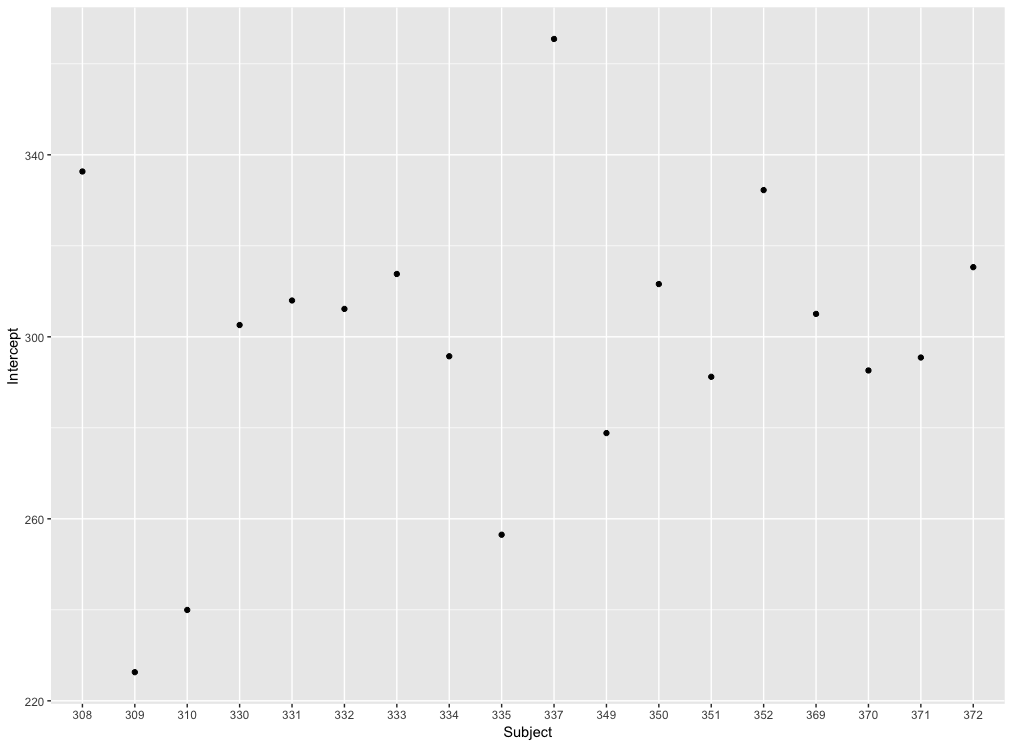
\includegraphics[width=4.5in]{./resources/random_intercepts.png}
\end{center}
\end{frame}

\begin{frame}[fragile]{Random Effects in R}
\footnotesize
\begin{minted}{R}
#This line create a dataframe for 18 hypothetical new subjects
#taking the estimated standard deviation reported in
#summary(m_avg)
new_subject <- data.frame(Subject = as.character(400:417),
  Intercept= fixef(m_avg)+rnorm(18,0,35.75),Status="Simulated")
reaction_subject$Status <- "Observed"
reaction_subject <- rbind(reaction_subject,new_subject)
#new plot
ggplot(reaction_subject,aes(x=Subject,y=Intercept,color=Status))+
  geom_point()+
  geom_hline(aes(yintercept = fixef(m_avg)[1],linewidth=1.5))

\end{minted}
\end{frame}

\begin{frame}%{Random Effects in R}
\begin{center}
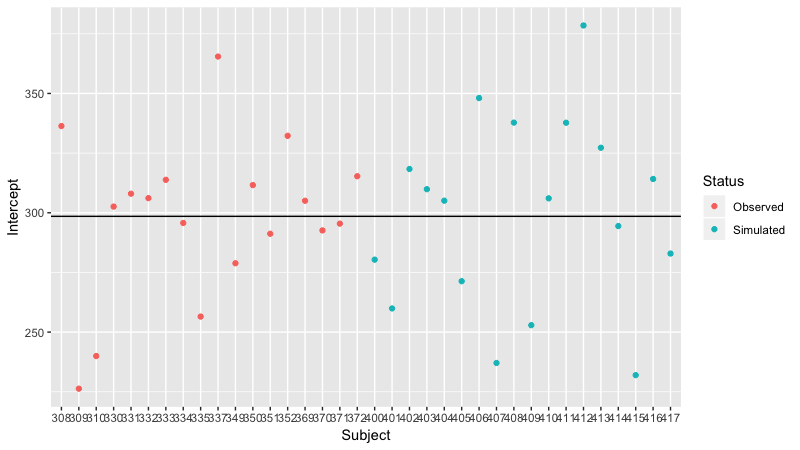
\includegraphics[width=5in]{./resources/random_intercepts2.png}
\end{center}
\end{frame}

\begin{frame}{Random Slope and Intercept / Random Coefficients}
\begin{align*}
y_{it} = \beta_i x_{it} + c_i + u_{it}
\end{align*}
\begin{itemize}
\item Can add a random slope term $\beta_i$ as well
\item This starts to get more useful
\item Parametric restrictions $\beta_i \sim N(0,\sigma_b^2)$ prevent $\beta_i$ realizations from getting too crazy.
\item Later we will think about parametrizing this further $\beta_i(z_i)$
\end{itemize}
\end{frame}




\begin{frame}[fragile]{Random Slope and Intercept R}
\tiny
\begin{minted}{R}
#fit the model
m_slp <- lmer(Reaction ~ Days + (Days | Subject), sleepstudy)
#the next line put all the estimated intercept and slope per
#subject into a dataframe
reaction_slp <- as.data.frame(t(apply(ranef(m_slp)$Subject,
  1,function(x) fixef(m_slp) + x)))
#to get the predicted regression lines we need one further
#step, writing the linear equation: Intercept + Slope*Days
#with different coefficient for each subject
pred_slp <- melt(apply(reaction_slp,1,function(x) x[1] + x[2]*0:9),
  value.name = "Reaction")
#some re-formatting for the plot
names(pred_slp)[1:2] <- c("Days","Subject")
pred_slp$Days <- pred_slp$Days - 1
pred_slp$Subject <- as.factor(pred_slp$Subject)

#plot with actual data
ggplot(pred_slp,aes(x=Days,y=Reaction,color=Subject))+
  geom_line()+
  geom_point(data=sleepstudy,aes(x=Days,y=Reaction))+
  facet_wrap(~Subject,nrow=3)
\end{minted}
\end{frame}

\begin{frame}%{Random Effects in R}
\begin{center}
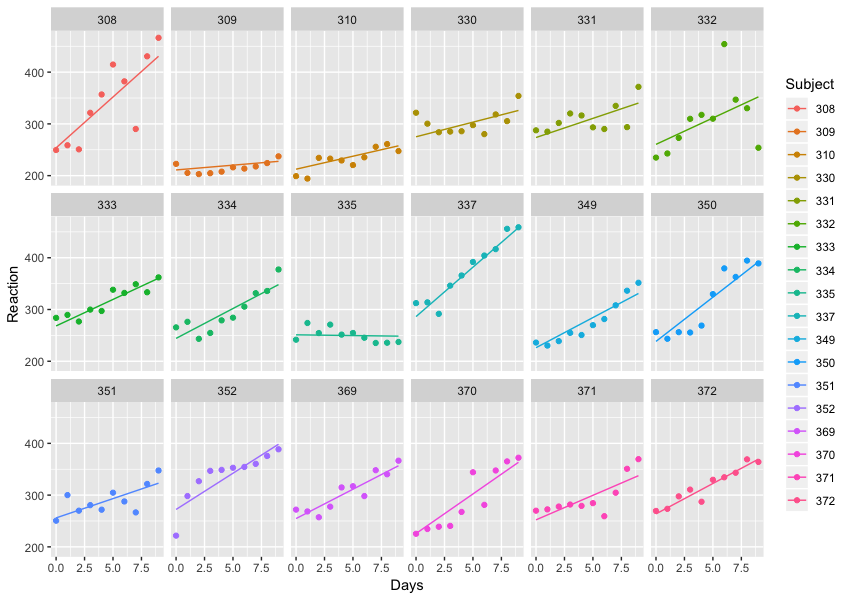
\includegraphics[width=4.8in]{./resources/random_slope_intercept.png}
\end{center}
\end{frame}

\begin{frame}{Control Variables vs. Variables of Interest}
We call a variable $W_i$ a control variable if:
\begin{align*}
E[u_i | X_i, W_i] = E[u_i | W_i]
\end{align*}
Consider the regression model
\begin{align*}
Y_i = \beta_0 + \beta_1 X_i + \beta_2 W_i + u_i
\end{align*}
\begin{itemize}
    \item $\beta_1$ has an interpreation
    \item $\widehat{\beta}_1$ is unbiased
    \item $\widehat{\beta}_2$ is potentially biased: something omitted might be correlated with $W_i$ and a determinant of $Y_i$. 
\end{itemize}
\end{frame}


\begin{frame}{Fixed Effects}
We could think about the same model but now instead of being part of the \alert{residual} $c_i$ is a dummy variable that we want to estimate a (fixed) coefficient on
\begin{align*}
y_{it} = \beta x_{it} + c_i + u_{it}
\end{align*}
Now we require that $E[u_{it}| \mathbf{X}_i , c_i] = 0$
\begin{itemize}
    \item Conditional on observing $c_i$ we have conditional mean independence property satisfied again.
    \item $c_i$ is just a conventional omitted variable: without it our estimate is \alert{biased}, include it in the regression and everything is fine.
\end{itemize}
\end{frame}


\begin{frame}{Fixed Effects as Controls}
\begin{align*}
y_{it} = \beta x_{it} + c_i + u_{it}
\end{align*}
A weaker condition is $E[u_{it}| \mathbf{X}_i , c_i] = E[u_{it}| c_i]$ but allowing $E[u_{it}| \mathbf{X}_i , c_i]\neq 0$
\begin{itemize}
\item Now the fixed effect functions only as a \alert{control}
\item We can't interpret $c_i$ directly, it just proxies for all of the things we don't see
\item Our estimates of $\hat{c}_i$ may be biased, but our estimtes of $\beta$ remain \alert{unbiased}.
\item There is \alert{NO} causal interpretation of fixed effects unless \alert{all variables} correlated with $Y_i$ and $c_i$ are in the regression equation.
\end{itemize}
\end{frame}

\begin{frame}{Fixed Effects: Within Estimator}
The fixed effects estimator
\begin{align*}
y_{it} = \beta x_{it} + c_i + u_{it}
\end{align*}
Is equivalent to the \alert{within estimator} 
\begin{align*}
(y_{it} - \overline{y}_i) = \beta (x_{it} - \overline{x}_i) + (u_{it} - \overline{u}_i)
\end{align*}
You should have learned about this last semester.\\
Also known as \alert{Absorb} / \alert{ Difference Out} / \alert{ Within Transform}
\end{frame}

\begin{frame}{Fixed Effects: LSDV Estimator}
The fixed effects estimator
\begin{align*}
y_{it} = \beta x_{it} + c_i + u_{it}
\end{align*}
Is also equivalent to the least squres dummy variables (LSDV) regression:
\begin{align*}
y_{it} = \beta x_{it} + \sum_{i=1}^N \gamma_i \cdot \mathbf{I}_{i} + u_{it}
\end{align*}
You should have learned about this last semester.
\end{frame}


\begin{frame}{Fixed Effects: Multicolinearity}
If we include a dummy (or fixed effect for every state we cannot estimate a constant term)
\begin{align*}
y_{it} = \alert{\beta_0} + \beta x_{it} + c_i + u_{it}
\end{align*}
\begin{itemize}
\item Most software will drop one fixed effect
\item Which fixed effect is dropped matters for $c_i$ but not for $\widehat{\beta}$.    
\end{itemize}
\end{frame}

\begin{frame}{Fixed Effects: Multi-way}
Often we want to include multiple dimensions of fixed effects
\begin{align*}
y_{it} =\beta x_{it} + c_i + c_t + u_{it}
\end{align*}
Two ways to do this
\begin{itemize}
\item Within transform the larger dimension $\rightarrow$ Include dummies for the smaller dimension
\item Transform the data in both dimensions using \alert{Frisch-Lovell-Waugh}.
\item Former when second dimension is small, latter when both are large
\end{itemize}
\end{frame}


\begin{frame}{High Dimensional Fixed Effects: Conlon and Rao} 
\begin{itemize}
 \item Suppose I want to incorporate \alert{store-upc} and \alert{store-week} FE using Nielsen Data.
\begin{itemize}
\item Around 500 weeks since 2006.
\item Around 3000+ UPCs in a category like distilled spirits or breakfast cereal.
\item Can easily find ourselves estimating 50,000+ fixed effects in a single dimension and several thousand in the other.
\end{itemize}
  \end{itemize}
\end{frame}



\begin{frame}{High Dimensional Fixed Effects}
There are several differencing algorithms for removing the fixed effects. For simplicitly let's assume there are two dimensions of fixed effects $N$ and $T$ where $N >> T$:
\begin{align*}
\tilde{y}_{it}&= y_{it} -\overline{y}_{i \cdot} - \overline{y}_{\cdot t}\\
\tilde{x}_{it}&= x_{it} -\overline{x}_{i \cdot} - \overline{x}_{\cdot t}
\end{align*}

\begin{itemize}
\item Could do \textit{iterative demeaning}: easy if $Cov(\overline{x}_{\cdot t},\overline{x}_{i \cdot})=0$. Otherwise hard.
\item Depends on \alert{graph structure} of FE. \alert{Sparse} FE are very difficult. \alert{Balanced Panels} are easy.
\item LSDV requires inverting the $(N+T) \times (N+T)$ matrix which can be difficult to impossible.
\end{itemize}
\end{frame}

\begin{frame}{FE in Dimension One}
\begin{align*}
\mathbf{Y} = \mathbf{Z} \beta + \mathbf{D} \alpha + \mathbf{u}
\end{align*}

Partition $\mathbf{X} = [\mathbf{Z} \mathbf{D}]$ where
\begin{align*}
\left[ \begin{array} { c c } { \mathbf { Z } ^ { \prime } \mathbf { Z } } & { \mathbf { Z } ^ { \prime } \mathbf { D } } \\ { \mathbf { D } ^ { \prime } \mathbf { Z } } & { \mathbf { D } ^ { \prime } \mathbf { D } } \end{array} \right] \left[ \begin{array} { l } { \beta } \\ { \alpha } \end{array} \right] = \left[ \begin{array} { c } { \mathbf { Z } ^ { \prime } \mathbf { Y } } \\ { \mathbf { D } ^ { \prime } \mathbf { Y } } \end{array} \right]\\
\end{align*}
Can be re-written
\begin{align*}
\left[ \begin{array} { c } { \mathrm { Z } ^ { \prime } \mathbf { Z } \beta + \mathbf { Z } ^ { \prime } \mathbf { D } \alpha = \mathbf { Z } ^ { \prime } \mathbf { Y } } \\ { \mathbf { D } ^ { \prime } \mathbf { Z } \beta + \mathbf { D } ^ { \prime } \mathbf { D } \alpha = \mathbf { D } ^ { \prime } \mathbf { Y } } \end{array} \right]
\end{align*}
And construct \alert{normal equations}
\begin{align*}
\left[ \begin{array} { c } { \beta = \left( \mathbf { Z } ^ { \prime } \mathbf { Z } \right) ^ { - 1 } \mathbf { Z } ^ { \prime } ( \mathbf { Y } - \mathbf { D } \alpha ) } \\ { \alpha = \left( \mathbf { D } ^ { \prime } \mathbf { D } \right) ^ { - 1 } \mathbf { D } ^ { \prime } ( \mathbf { Y } - \mathbf { Z } \beta ) } \end{array} \right]
\end{align*}
\end{frame}


\begin{frame}{FE in Dimension One}
Idea is to \alert{Iterate on Normal Equations}
\begin{align*}
\left[ \begin{array} { c } { \beta = \left( \mathbf { Z } ^ { \prime } \mathbf { Z } \right) ^ { - 1 } \mathbf { Z } ^ { \prime } ( \mathbf { Y } - \mathbf { D } \alpha ) } \\ { \alpha = \left( \mathbf { D } ^ { \prime } \mathbf { D } \right) ^ { - 1 } \mathbf { D } ^ { \prime } ( \mathbf { Y } - \mathbf { Z } \beta ) } \end{array} \right]
\end{align*}
In one dimension this is silly because we just do the \alert{within trnasform}. But this idea extends to higher dimensions.
\end{frame}

\begin{frame}{FE in two (or more) Dimensions}
\begin{align*}
\left[ \begin{array} { c } { \beta = \left( \mathbf { Z } ^ { \prime } \mathbf { Z } \right) ^ { - 1 } \mathbf { Z } ^ { \prime } \left( \mathbf { Y } - \mathbf { D } _ { 1 } \alpha - \mathbf { D } _ { 2 } \gamma \right) } \\ { \alpha = \left( \mathbf { D } _ { 1 } ^ { \prime } \mathbf { D } _ { 1 } \right) ^ { - 1 } \mathbf { D } _ { 1 } ^ { \prime } \left( \mathbf { Y } - \mathbf { Z } \beta - \mathbf { D } _ { 2 } \gamma \right) } \\ { \gamma = \left( \mathbf { D } _ { 2 } ^ { \prime } \mathbf { D } _ { 2 } \right) ^ { - 1 } \mathbf { D } _ { 2 } ^ { \prime } \left( \mathbf { Y } - \mathbf { Z } \beta - \mathbf { D } _ { 1 } \gamma \right) } \end{array} \right]
\end{align*}
Note
\begin{itemize}
\item We residualize $\mathbf{Y}$
\item We don't mess with $\mathbf{X}$ at all
\item But we run many regressions
\end{itemize}
\end{frame}

\begin{frame}{Pass Through Regressions}
\begin{eqnarray*}
\Delta p_{jt} =  \beta_0 + \alert{\rho(X_{jt}, \Delta \tau_{jt}) } \Delta \tau_{jt} + \beta_2 \Delta c_{jt} + B\Delta X_{jt} + \alpha_j + \gamma_t + \epsilon_{jt}
\end{eqnarray*}
\begin{itemize}
%\item Estimation in price levels rather than logs.
\item $\gamma_t$ is typically month $+$ year FE.
\item $\alpha_j$ is a product-specific trend in price.
\item We estimate these in first differences, and vary the time horizon (1 month, 3 months, 6 months).
\begin{itemize}
%Ask Conlon
%\item Sometimes we condition on cases when the price is the same for the entire period.
\item Sometimes we  examine only firms which change their prices.
\end{itemize}
\end{itemize}
\end{frame}

\begin{frame}[fragile]{R Code}
\begin{minted}{R}
require(lfe)
fe1<-felm(data=data,delta_p~ delta_t:my_spectax | stateupc+statemonth+stateyear | 0 | stateupc,weights=data$weights_q)
\end{minted}
\end{frame}


\begin{frame}{Pass-Through:  Taxes to Retail Prices, CT}
\tiny
\begin{table}[htp]
\begin{center}
\begin{tabular}{l l l l l l l } \hline
& \multicolumn{3}{c}{All Retailers} & \multicolumn{3}{c}{$\Delta$ Retail Price$ \neq 0$} \\ 
 $\Delta$ Retail Price & 1m & 3m & 6m & 1m & 3m & 6m \\   
 & (1) & (2) & (3) & (4) & (5) & (6)  \\  
\hline
$\Delta$ Tax & 1.533*** & 1.257*** & 1.013*** & 3.096*** & 2.301*** & 2.016*** \\
& (0.271) & (0.202) & (0.264) & (0.706) & (0.479) & (0.553) \\ \hline
$\Delta$ Tax*I[size=750mL] & 1.168*** & 1.900*** & 2.084*** & 3.191** & 3.822*** & 4.072*** \\
& (0.432) & (0.387) & (0.503) & (1.577) & (0.899) & (1.144) \\
$\Delta$ Tax*I[size=1L] & 2.146*** & 1.833*** & 1.586*** & 5.550*** & 3.376*** & 3.553*** \\
& (0.650) & (0.383) & (0.470) & (1.663) & (0.920) & (1.132) \\
$\Delta$ Tax *I[size=1.75L]  & 1.520*** & 1.154*** & 1.009*** & 2.985*** & 2.191*** & 2.027*** \\
& (0.309) & (0.227) & (0.263) & (0.718) & (0.502) & (0.570) \\ \hline
Observations & 460,116 & 437,057 & 410,288 & 75,227 & 113,098 & 142,220\\
Product FE & Yes & Yes & Yes & Yes & Yes & Yes \\  \hline
\end{tabular}
\end{center}
\begin{tablenotes}
\footnotesize \item \tiny Note: All regressions are weighted by 2011 Nielsen units and include month and year fixed effects. Standard errors are clustered at the UPC level.
\end{tablenotes}
\end{table}
\end{frame}



\begin{frame}[fragile]{High Dimensional FE Examples: Backus, Conlon Sinkinson (2019)}
\footnotesize
\begin{align*}
\kappa_{fg,t} &= \beta_1 \log \text{Market Cap}_{f,t} + \beta_2\frac{1}{\text{Retail Share}_{f,t}} + \beta_3\text{Indexing}_{f,t} +\\
&\beta_4 \text{Indexing}_{f,t}^2 + \beta_5 \text{Indexing}_{f,t}^3 \beta_5 BlackRock_{f,t} + \beta_6 Vanguard_{f,t} + \beta_7 StateStreet_{f,t} 
 + c_{f,g} + c_t + u_{f,g,t}
\end{align*}

\tiny
\begin{minted}{R}
require(lfe)
fe4<-felm(data=data,kappa~I(1/(1-retail_share)) + I(log(market_cap))+ poly(normalized_l2,3) + 
BlackRock  + Vanguard + StateStreet| pair + quarter | 0 | pair)
\end{minted}
\end{frame}

\begin{frame}
\tiny
\begin{center}
\begin{tabular}{@{\extracolsep{5pt}}lccccc} 
\toprule
\\[-1.8ex] & (1) & (2) & (3) & (4) & (5)\\ 
\midrule
$\frac{1}{1-r_{f,t}}$& 0.314$^{*}$ & 0.301$^{*}$ & 0.304$^{*}$ & 0.305$^{*}$ & $-$0.172$^{*}$ \\ 
  & (0.001) & (0.001) & (0.001) & (0.001) & (0.001) \\ 
$\frac{1}{IHHI_{f,t}}$&  &  &  &  & 45.505$^{*}$ \\ 
  &  &  &  &  & (0.083) \\ 
$\log$(market cap)$_{f,t}$ & 0.081$^{*}$ & 0.078$^{*}$ & 0.077$^{*}$ & 0.077$^{*}$ & 0.029$^{*}$ \\ 
  & (0.0003) & (0.0003) & (0.0003) & (0.0003) & (0.0003) \\ 
  & & & & & \\ 
Indexing$_{f,t}$ & 0.964$^{*}$ & 1.079$^{*}$ &237.411$^{*}$  &237.069$^{*}$  & 1.253$^{*}$ \\ 
  & (0.004) & (0.004) & (1.065) & (1.069) & (0.004) \\ 
Indexing$_{f,t}^2$  &  &  & $-$68.704$^{*}$ &$-$70.900$^{*}$  &  \\ 
  &  &  & (0.656) &(0.636)  &  \\ 
Indexing$_{f,t}^3$ &  &  &  & $-$19.064$^{*}$ &  \\ 
  &  &  &  & (0.520) &  \\ 
$\beta_{f,s,t}$ BlackRock &  & $-$0.406$^{*}$ & $-$0.333$^{*}$ & $-$0.344$^{*}$ & $-$0.288$^{*}$ \\ 
  &  & (0.007) & (0.007) & (0.007) & (0.006) \\ 
$\beta_{f,s,t}$ Vanguard &  & $-$0.311$^{*}$ & $-$0.234$^{*}$ & $-$0.229$^{*}$ & $-$1.226$^{*}$ \\ 
  &  & (0.016) & (0.016) & (0.016) & (0.014) \\ 
$\beta_{f,s,t}$ StateStreet &  & $-$0.509$^{*}$ & $-$0.420$^{*}$ & $-$0.414$^{*}$ & $-$0.275$^{*}$ \\ 
  &  & (0.014) & (0.014) & (0.014) & (0.012) \\ 
  \midrule
 \textit{N} & 17,397,247 & 17,397,247 & 17,397,247 & 17,397,247 & 17,397,247 \\ 
R$^{2}$ & 0.735 & 0.735 & 0.737 & 0.737 & 0.797 \\ 
\bottomrule
\end{tabular} 
\end{center}
\end{frame}




\begin{frame}{Employment}
\begin{center}
%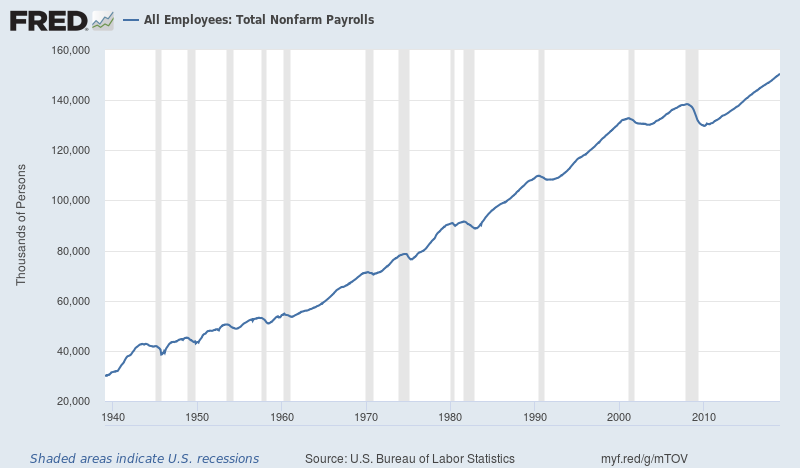
\includegraphics[width=5in]{./resources/nonfarm_level.png}
\end{center}
\end{frame}

